\todo{CS4002}
\todo[color=blue!40]{CS4003}
\todo[color=green!40]{CS4004}

En este capítulo se introducen los conceptos necesarios para el desarrollo de la propuesta de investigación. Por un lado, se describe la etapa de  correspondencia y los métodos involucrados en el proceso como \textit{pointnet} y redes neuronales siameses (SNN). Por otro lado, se explica la etapa de alineación, y los métodos de \textit{deep closest point} (DCP) y \textit{deep global registration} (DGR).

\section{Correspondencia}

La correspondencia de objetos 3D consiste en mapear los puntos de un modelo $X$ en una posición $M$ a una posición $N$ a través de una transformación $T$. La transformación se define formalmente en la ecuación \ref{eq:3}, donde $f$ y $g$ son los descriptores de $M$ y $N$ respectivamente \cite{17}.

\begin{equation} \label{eq:3}
    f:M \xrightarrow{} \mathbb{R}^n; \ \ \ \ \ T_F (f) = g:N \xrightarrow{} \mathbb{R}^n
\end{equation}

De manera similar, con una transformación diferente, el problema entre posiciones se convierte en el mapeo de una cara fracturada $X$ a una cara $Y$. Entonces, la correspondencia en el reensamblaje consiste en emparejar los fragmentos de un conjunto inicial de tal manera que se puedan unir y formar un nuevo fragmento, como se muestra en la figura \ref{fig:correspondencia} \cite{2}. 

\begin{figure}[!h]
    \centering
     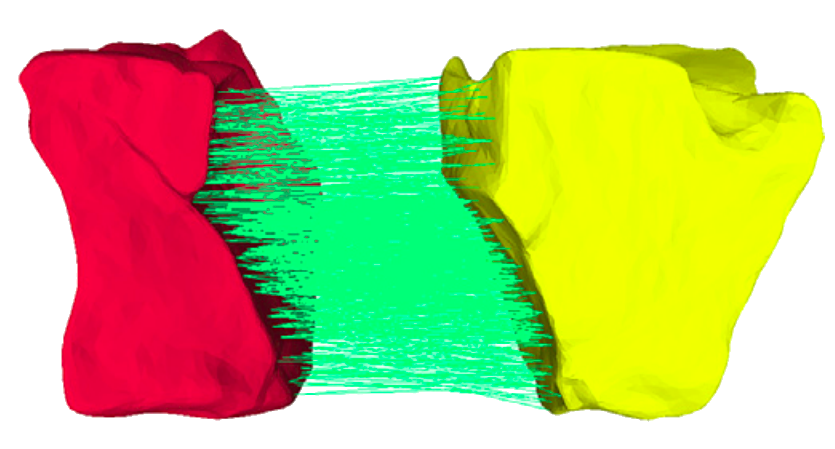
\includegraphics[scale=0.18]{images/correspondencia.png}
    \caption{Correspondencia entre fragmentos \cite{5}}
    \label{fig:correspondencia}
\end{figure}

% \subsection{Curvatura}


\subsection{\textit{Pointnet}}
Es una arquitectura de red neuronal que recibe como entrada una nube de puntos para resolver tareas como clasificación de objetos o segmentación de partes, tal como se muestra en la figura \ref{fig:pointnet}. Primero, se inicia con una transformación de la entrada con una T-net para asegurar que sea invariante a transformaciones como rotación o traslación. Segundo, se extraen los vectores característicos de los puntos y se aplica una segunda transformación. Tercero, se emplea un \textit{multilayer perceptron} (MLP) y un \textit{max pooling} para asegurar que sea invariante al orden de los puntos de entrada. Con el vector de características globales obtenidas en el paso anterior, podemos agregar una MLP para clasificar objetos, o agregar las características locales para resolver la tarea de segmentación \cite{14}.

\begin{figure}[!h]
    \centering
     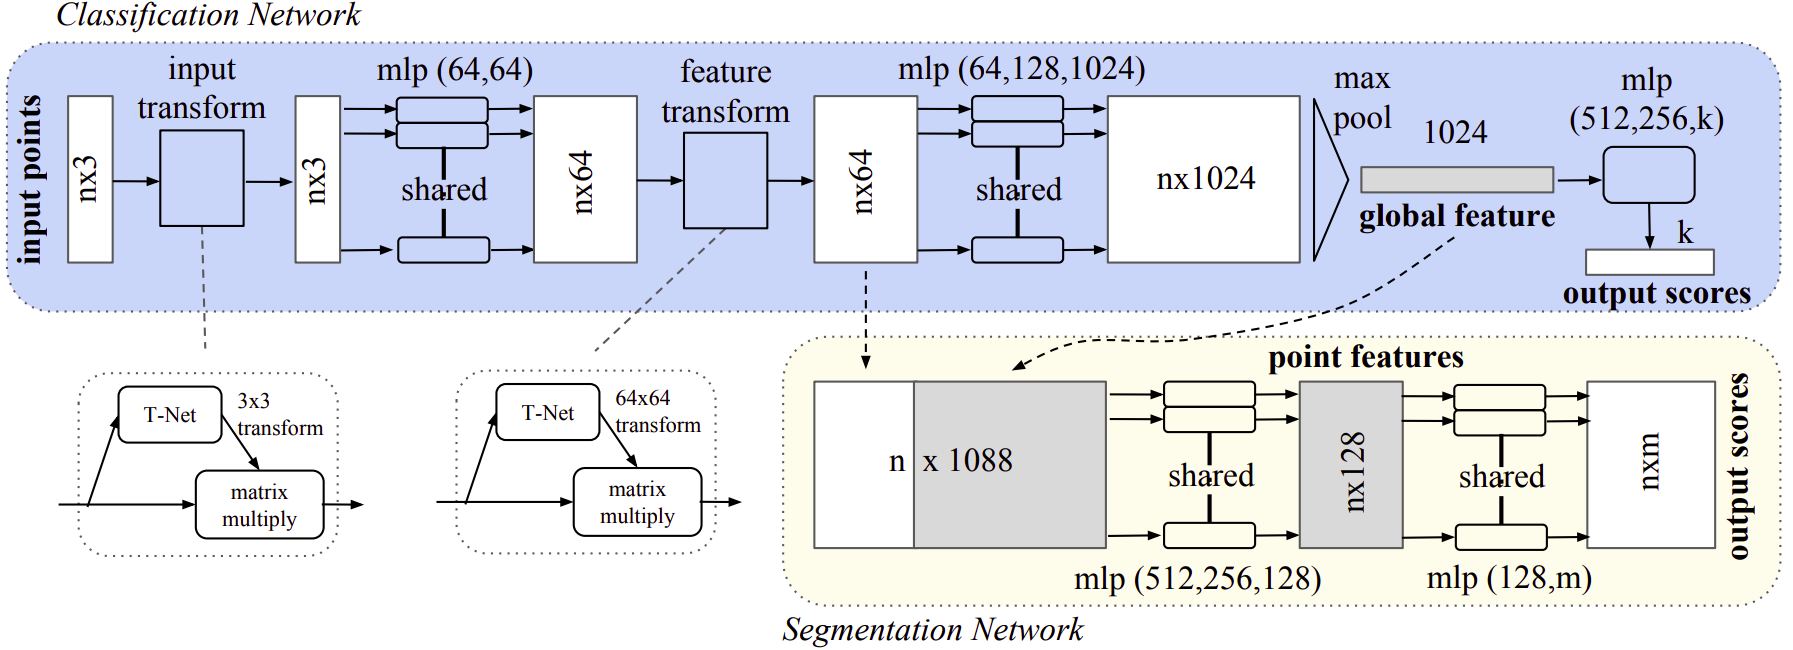
\includegraphics[scale=0.19]{images/pointnet.png}
    \caption{Arquitectura de la \textit{Pointnet} \cite{14}}
    \label{fig:pointnet}
\end{figure}

\subsection{Redes neuronales siamesas (SNN)}
Es una arquitectura compuesta por dos subredes neuronales idénticas que comparten el mismo conjunto de pesos. En la figura \ref{fig:snn} se muestra como cada red recibe una entrada diferente, de la cual extrae su respectivo vector característico. A continuación, los vectores característicos se comparan para determinar su similitud semántica a través de una función de pérdida de contraste. Además, SNN puede ser usado para resolver tareas como la verificación de imágenes, y detección de anomalías \cite{15}. 

\begin{figure}[!h]
    \centering
     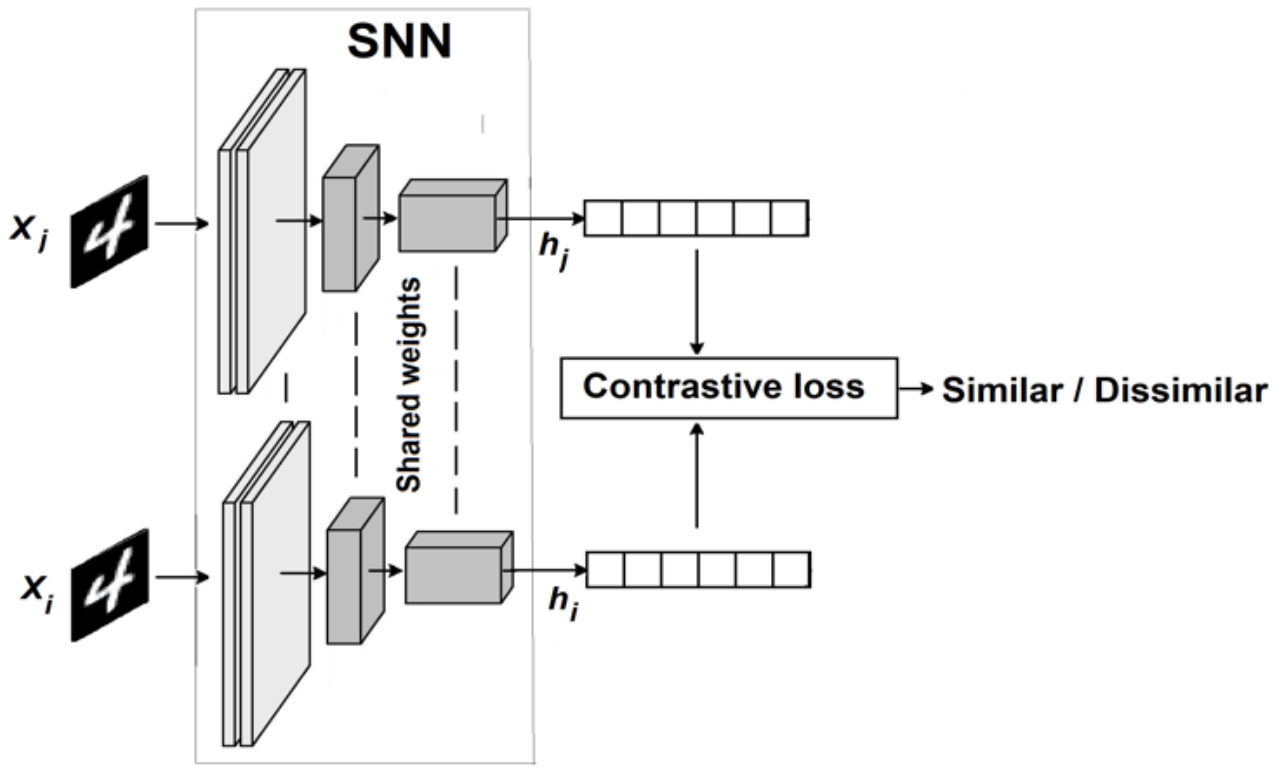
\includegraphics[scale=0.17]{images/snn.png}
    \caption{Arquitectura de la \textit{SNN} \cite{15}}
    \label{fig:snn}
\end{figure}



\section{Alineación}
La alineación de objetos 3D consiste en encontrar la transformación rígida, compuesta por un vector de rotación $\hat{R}$ y un vector de traslación  $\hat{t}$, que minimiza la distancia entre las nubes de puntos $X$ y $Y$, dado el conjunto de correspondencias $M$. Formalmente, el problema está definido por la ecuación \ref{eq:4}, donde $g$ representa la transformación, y $d$ es el error entre $X$ y $Y$ transformado \cite{9}. 

\begin{equation} \label{eq:4}
    \argmin_{\hat{R}, \hat{t}}||d(X, g(Y))||^2_2 \ ; \ \ \ \ \ g(Y) = \hat{R}Y + \hat{t}
\end{equation}

En el problema de reensamblaje, la alineación también debe minimizar el \textit{overlapping} entre las nubes de puntos para hallar la mejor transformación. Además, la alineación puede tener dos etapas: una alineación global y una local \cite{2}. En la figura \ref{fig:alineacion}, se muestra la alineación entre dos caras de los fragmentos $X$ y $Y$, donde la transformación $T$ se aplica sobre el fragmento $X$.

\begin{figure}[!h]
    \centering
     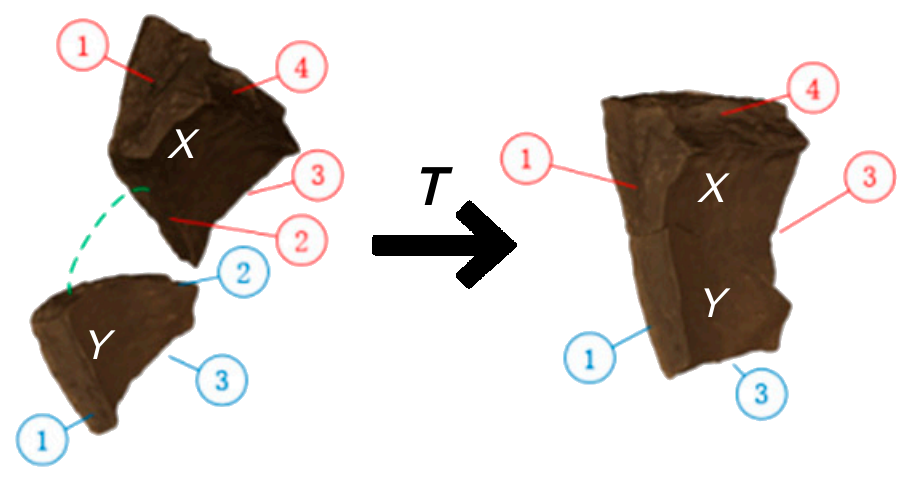
\includegraphics[scale=0.19]{images/alineacion.png}
    \caption{Alineación entre fragmentos \cite{6}}
    \label{fig:alineacion}
\end{figure}


% \subsection{\textit{Principal Component Analysis} (PCA)}
\subsection{\textit{Deep Closest Point} (DCP)}
Es un método de alineación basado en \textit{deep learning} conformado por tres módulos. El primero es una red neuronal que recibe nubes de puntos para extraer un \textit{embedding} que represente las características relevantes. El segundo es un módulo basado en atención con una capa de generación de correspondencias para aproximar el emparejamiento entre los vectores de características de ambas entradas. El tercero es una capa de descomposición de valor singular diferenciable (SVD) para extraer la transformación final. La figura \ref{fig:dcp} ilustra el proceso mencionado.
\begin{figure}[!h]
    \centering
     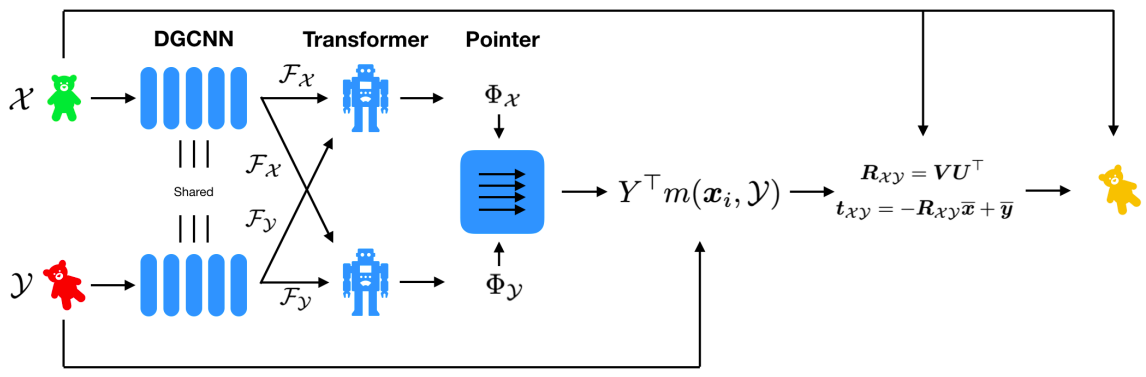
\includegraphics[scale=0.3]{images/dcp.png}
    \caption{Arquitectura de la \textit{DCP} \cite{16}}
    \label{fig:dcp}
\end{figure}

\subsection{\textit{Deep Global Registration} (DGR)}
Es un método de alineación compuesto por tres módulos principales: la extracción y predicción, el análisis de distribución balanceado y la optimización final. La figura \ref{fig:dgr} ilustra el proceso mencionado a alto nivel.

\begin{figure}[!h]
    \centering
    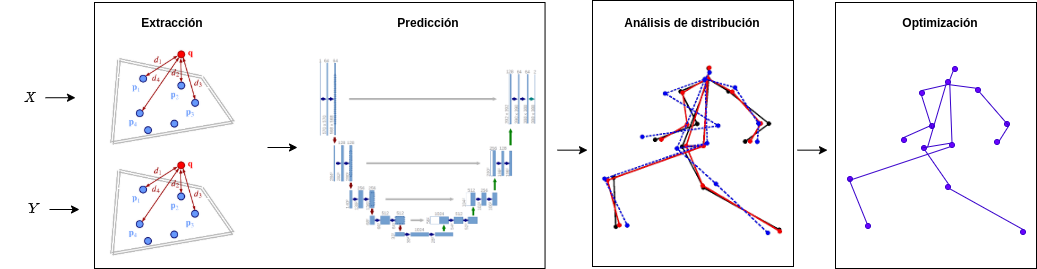
\includegraphics[scale=0.325]{images/dgr.png}
    \caption{\textit{Pipeline} de DGR}
    \label{fig:dgr}
\end{figure}

\begin{enumerate}
    \item Extracción y predicción. Este módulo tiene 3 etapas. En la primera, se extraen los vectores característicos de las nubes de puntos $X$ y $Y$. En la segunda, se genera un conjunto $M$ con las correspondencias $(x_i, y_i)$, donde $y_i$ es el vecino más cercano de $x_i$ en el espacio de vectores característicos. En la tercera, se utiliza una red neuronal convolucional (CNN) con estructura de U-net para predecir el \textit{likelihood} de las correspondencias entre puntos en $M$ \cite{10}.
    
    \item Análisis de distribución balanceado. El método minimiza el error cuadrático medio ponderado entre los puntos de correspondencia (\ref{eq:1}), donde los pesos $w$ son el \textit{likelihood} obtenido en el módulo anterior. Este método genera un vector de rotación $\hat{R}$ y un vector de traslación $\hat{t}$ \cite{10}.
    \begin{equation} \label{eq:1}
        \argmin_{\hat{R}, \hat{t}}\frac{1}{N}\sum_{(i, j) \in M} w(i,j) ||x_{i} - (\hat{R}y_{j} + \hat{t})||^{2}
    \end{equation}
    
    \item Optimización. El módulo refina la alineación a través de la minimización de una función de pérdida robusta \ref{eq:2}. Además, se utiliza un optimizador de descenso de gradiente como Adam o SGD para lograr la convergencia de los vectores de rotación $\hat{R}$ y traslación $\hat{t}$ \cite{10}.
    \begin{equation} \label{eq:2}
        loss = \sum_{i,j \in M} \phi(w(i,j)) \ L(x_i, \hat{R}y_{j} + \hat{t})
    \end{equation}
\end{enumerate}

\hfill\break
\indent En este capítulo, se definieron conceptos importantes como correspondencia y alineación dentro del proceso de reensamblaje. Además, se revisaron métodos relevantes para cada sub problema y su respectiva arquitectura. 

\hfill \break

Marco Teórico:

Descriptores:
...

Correspondencia
Alineación

Redes neuronales aplicadas a modelos 3D:
...


Revisión de la Literatura:

Reensamblaje
....

Correspondencia
...

Alineación
...
